The laboratory prototypes, which have been developed by Valencia research group in the framework of Tritium project, are detailed in this report. 

The Tritium detector are focused on monitoring of low radiactive tritium activities in water which is released for nuclear power plants. It is based on the deteccion of tritium radiation by scintillator fibers which will be read out by several photosensors (PMTs or SiPM arrays).

The fibers, which have been used in all prototypes, were buying in Saint-Gobain company, model BCF-12, whose diameter is $1~\mm$. In all the cases these fibers were cutted and polished at a distance of $20~\cm$. 

For the cutting process, the device, which is shown in the figure \ref{fig:Cuttingdevice}, was developed and built in the IFIC and the results was checked to the microscope.

\begin{figure}[htb]
\centering
{
%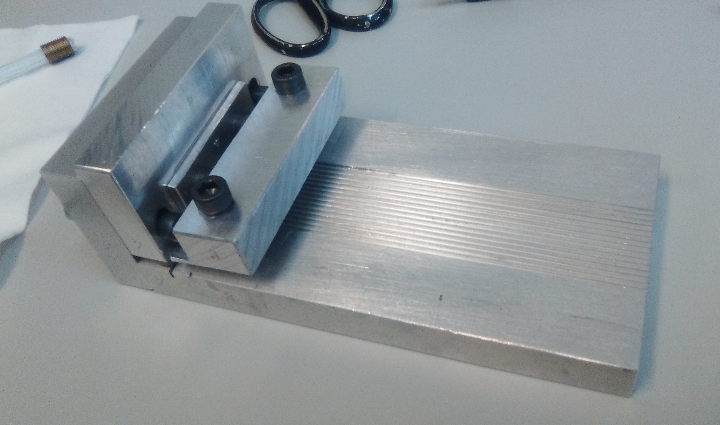
\includegraphics[scale=0.25]{Guillotina1.png} 
}
\caption{Cutting device \label{fig:Cuttingdevice}}
\end{figure} 

For the polishing process, the machine, which is shown in figure \ref{fig:PolishingMachine}, was developed and built at IFIC. This machine is controlled with arduino technology and it reproduces and automates the manual method recommended by Saint-Gobain. 

\begin{figure}[htb]
\centering
{
%\includegraphics[scale=0.25]{PolishingMachine.png} 
}
\caption{Polishing machine \label{fig:PolishingMachine}}
\end{figure} 

The results of this polishing process were verified under a microscope (figure \ref{fig:VisualResultPolish}) and with measurements of the light collection (figure \ref{fig:ResultPolish}). 

\begin{figure}[htbp]
\centering
\subfigure[Final face of the fiber before the polishing process \label{fig:VisualBeforePolish}]{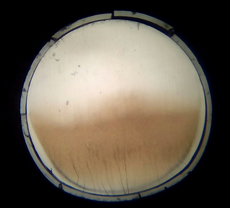
\includegraphics[width=60mm]{./Figuras/NoPolished.png}}\hspace{10mm}
\subfigure[Final face of the fiber after the polishing process \label{fig:VisualAfterPolish}]{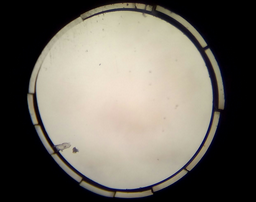
\includegraphics[width=70mm]{./Figuras/Polished.png}}
\caption{Visual result of the polishing process under the microscope} \label{fig:VisualResultPolish}
\end{figure}

\begin{figure}[htbp]
\centering
\subfigure[Measurement of the light produced in a bunch of $25$ fibers of $20~\cm$ due to the \ce{^{90}Sr} source \label{fig:SrPolish}]{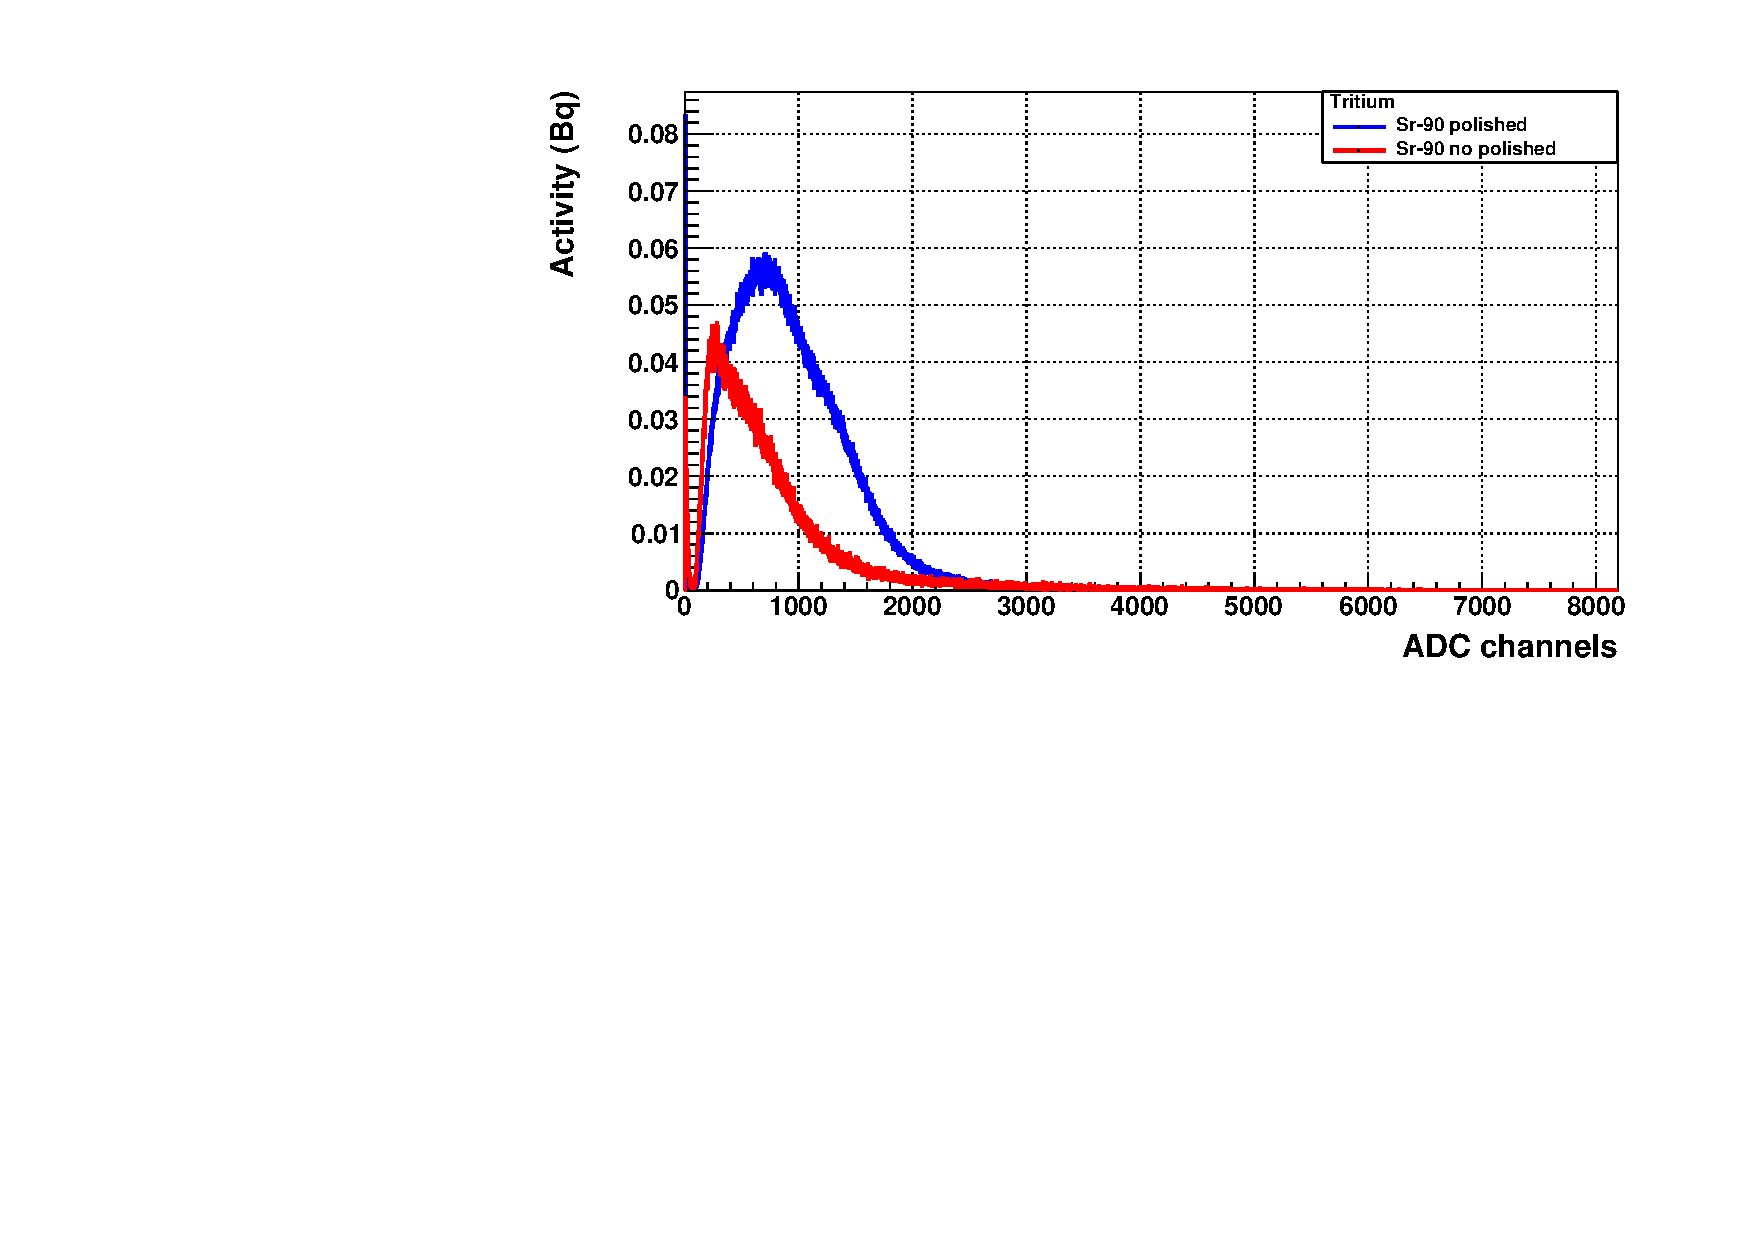
\includegraphics[width=77mm]{./Figuras/Sr_90.pdf}}
\subfigure[Measurement of the light produced in a bunch of $25$ fibers of $20~\cm$ due to the \ce{^{60}Co} source \label{fig:CoPolish}]{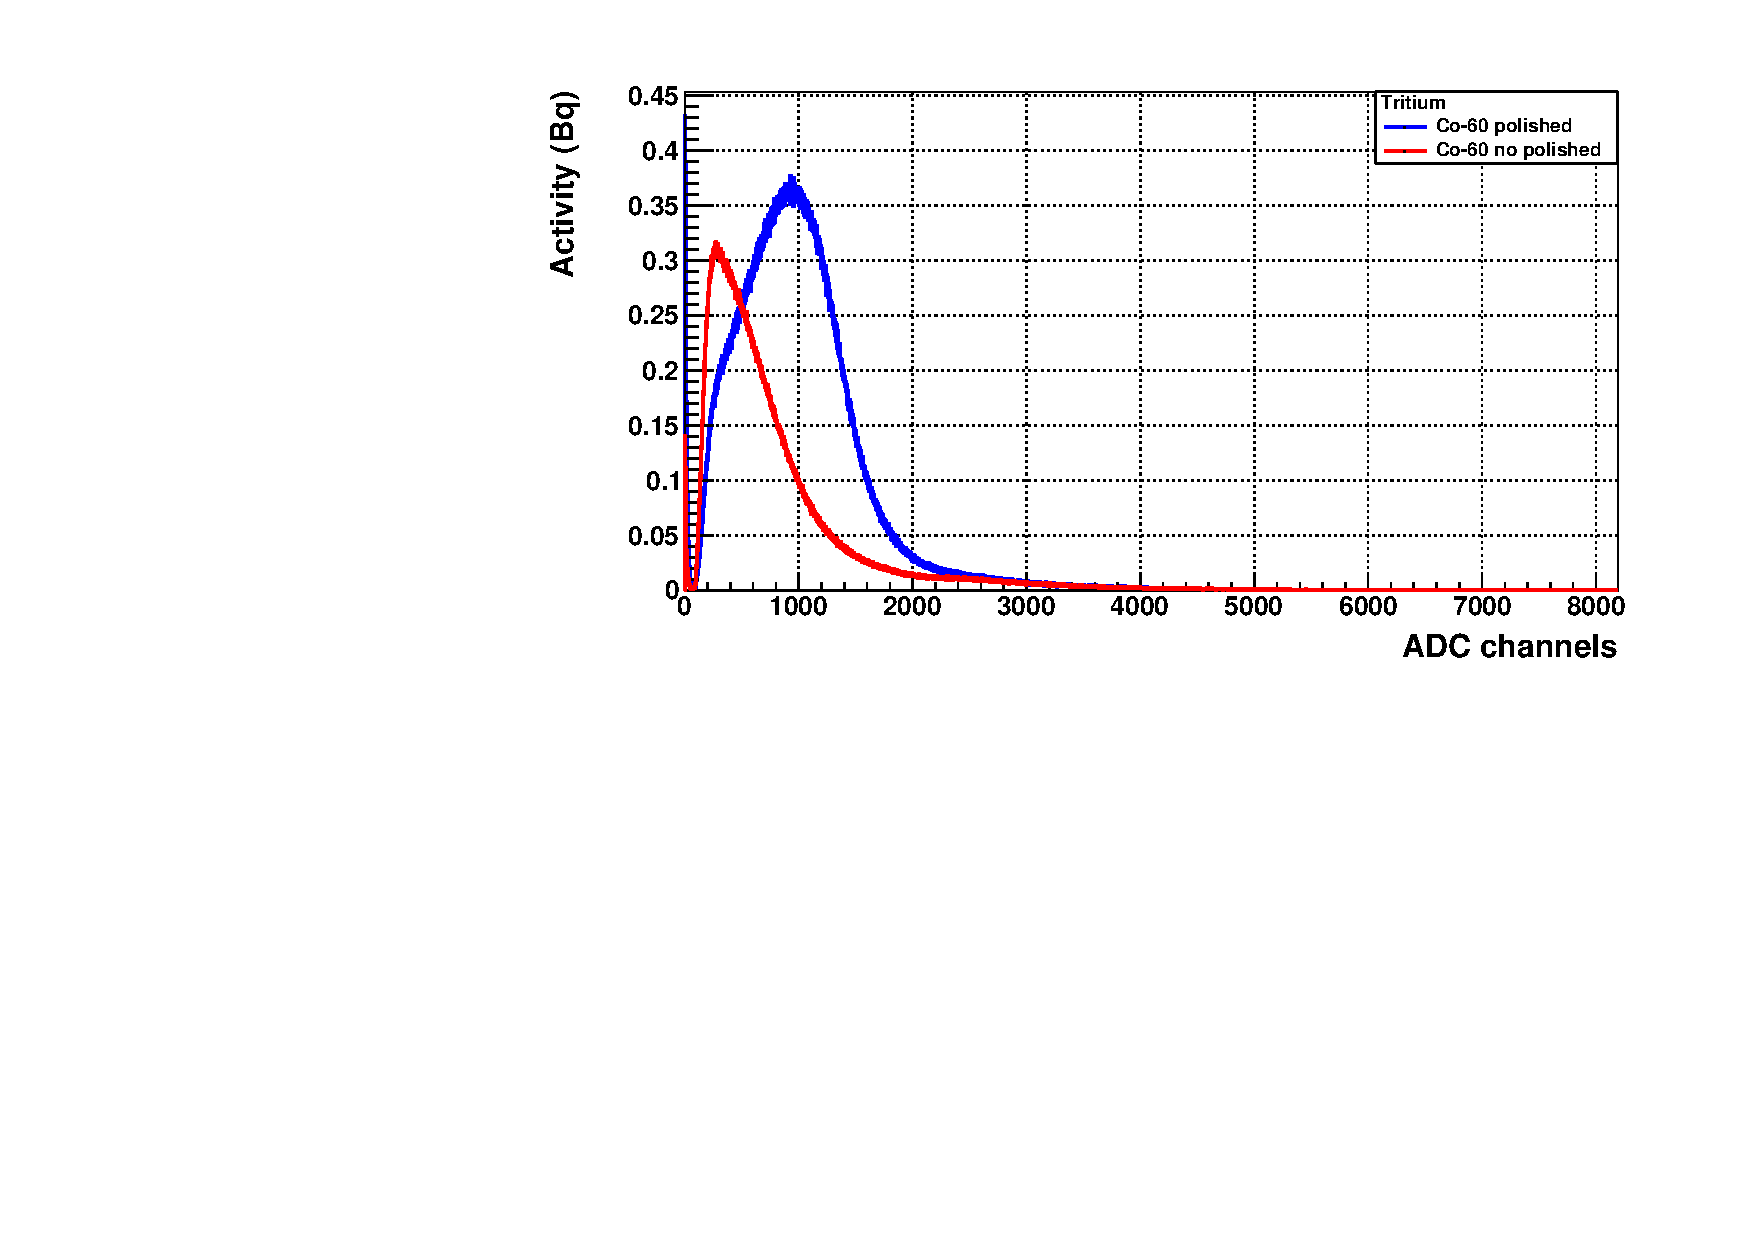
\includegraphics[width=77mm]{./Figuras/Co_60.pdf}}
\caption{Cuantification of the improvement of polishing process} \label{fig:ResultPolish}
\end{figure}

From this measurements the improvement in the light collection was quantified in around $50\%$ for $\beta$ radiation, as you can see in the table \ref{TablePolish}

\begin{table}
\centering
\begin{tabular}{l | c | c | c | c}
Source & Not polished & Polished & Improvement\\
\hline \hline
Sr-90 & 33 & 64  & 48.44 \% \\ 
Co-60 & 243 & 424 & 74.49 \% 
\end{tabular}
\caption{Counts/second due to each source \label{TablePolish}}
\end{table}

We have to take into account that in the final detector the water will flow through the detector, but it is not necessary for laboratory tests. The laboratory prototypes will be water hermetic to reduce the difficulty of these prototypes since the security requirements are strong due to the high activities contained in them.

The different prototypes, which have been created in Valencia, were filled following the same protocol which was developed in the IFIC. This protocol is explained in the seccion \ref{sec:FillInPrototypes}. All measurements were made inside a special black box which is light tight

In this work we will discuss the problems that was found in each prototype and how the next version overcomed these problems. On top of that, we will speak about the improvements that was included in each prototype and how it affect to our detector.